%%%%%%%%%%%%%%%%%%%%%%%%%%%%%%%%%%%%%%%%%%%%%%%%%%%%%%%%
%%%%%%%%%%%%%%%%%%%%%%%%%%%%%%%%%%%%%%%%%%%%%%%%%%%%%%%%
\section{Supervised Learning}
\label{ml:supervised}

In supervised learning a model is trained over many known examples
to use input features $\mathbf{X}$ to make a prediction \yhat about the true value $y$.
During the training process parameters $\beta$ of
the model are adjusted to minimize a two-part objective function,
$\text{obj}\left(\beta\right) = L\left(\beta\right) + \Omega\left(\beta\right)$.
The training loss $L\left(\beta\right)$ measures the model's predictive performance
while $\Omega\left(\beta\right)$ is a regularization term to penalize model complexity.
Note that $L$ is a measure of the model's bias and $\Omega$ is a measure of its variance,
so $\text{obj}\left(\beta\right)$ captures both parts of the bias-variance tradeoff \cite{HastieTF09}.

%%%%%%%%%%%%%%%%%%%%%%%%%%%%%%%%%%%%%%%%%%%%%%%%%%%%%%%%
\subsection{Loss Functions}
\label{ml:supervised:loss_functions}

\subsubsection{Binary Logistic}
\label{ml:supervised:loss_functions:binary_logistic}

In two class, signal $y=1$ and background $y=0$, classification problems the binary logistic function is an appropriate choice of $L$:

\begin{equation} \label{eq:binary_logistic}
L = \sum_{i} \left[y_{i} \ln\left(1 + \exp(-\yhat_{i})\right) +\left(1-y_{i}\right) \ln\left(1 + \exp(\yhat_{i})\right)\right].
\end{equation}

% TODO add more on the information theory aspect

% TODO add more loss functions

%%%%%%%%%%%%%%%%%%%%%%%%%%%%%%%%%%%%%%%%%%%%%%%%%%%%%%%%
\subsection{N{a\"i}ve Bayes Classification}
\label{ml:supervised:Bayes}
% TODO

%%%%%%%%%%%%%%%%%%%%%%%%%%%%%%%%%%%%%%%%%%%%%%%%%%%%%%%%
\subsection{\texorpdfstring{$k$}{k}-Nearest Neighbors (\texorpdfstring{$k$}{k}-NN)}
\label{ml:supervised:kNN}
% TODO
% TODO also talk about collaborative filtering

%%%%%%%%%%%%%%%%%%%%%%%%%%%%%%%%%%%%%%%%%%%%%%%%%%%%%%%%
\subsection{Support Vector Machines (SVM)}
\label{ml:supervised:SVM}
% TODO

%%%%%%%%%%%%%%%%%%%%%%%%%%%%%%%%%%%%%%%%%%%%%%%%%%%%%%%%
\subsection{Decision Trees, \ie Classification and Regression Trees (CART)}
\label{ml:supervised:CART}

A basic classifier can be created from a tree of selections on $\mathbf{X}$ designed to
separate the classes at each branch.
Such a model is known as a classification and regression tree (CART) \cite{Breiman:2253780}
and a simple example can be found in \cref{ml:supervised:CART:small_example_CART}.
As the splits are just selections on the input variables,
they are --- somewhat --- possible to understand,
and conveniently do not need any kind of feature scaling, unlike other methods.
To make a prediction for an event the tree and its branches are traversed
until the event lands in one of the weighted leaves.
The weight of the leaf $w$ is positive (negative) for signal-like (background-like) events.
A logistic function is used to properly transform $w$ into an output score
$\yhat = 1 /\left(1+e^{-w}\right)$ within $0 < \yhat < 1$.

\begin{figure}[H]
\centering
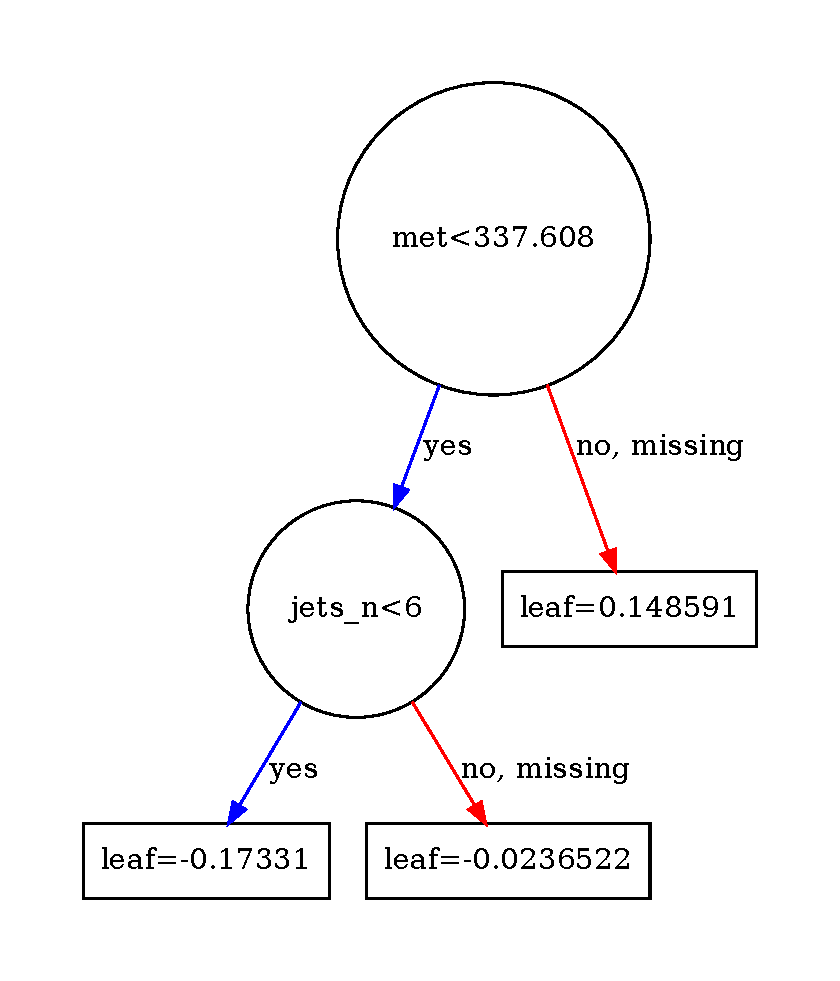
\includegraphics[width=0.4\textwidth]{figures/ml/tree7_g2000_n1200.pdf}
\caption{
Simple classification and regression tree (CART).
Signal-like (background-like) events receive positive (negative) weights in the leaves.
}
\label{ml:supervised:CART:small_example_CART}
\end{figure}

% TODO include gini impurity / importance

%%%%%%%%%%%%%%%%%%%%%%%%%%%%%%%%%%%%%%%%%%%%%%%%%%%%%%%%
\subsection{Boosted Decision Trees (BDT)}
\label{ml:supervised:BDT}

Individual CARTs are rather poor and limited models
in terms of the behaviors they can successfully predict.
However, by taking an ensemble of $K$ complementary trees, \ie boosting \cite{FREUND1997119,friedman2000},
and summing each CART's individual weight $w_{k}$ a much more flexible BDT\footnote{As the leaf weights
are reals rather than integer classes this approach may be better described as a boosted regression tree,
and can indeed handle regression problems without the logistic function.} is formed.
The component trees of a BDT are generated by iteratively adding new trees $f_{k}\left(x_{i}\right)$ to those which came before \cite{XGBoost},

\begin{equation} \label{eq:boosting}
\begin{aligned}
\hat{y}^{\left(0\right)} &= 0\,, \\
\hat{y}^{\left(1\right)} &= f_1\left(\mathbf{X}\right) = \hat{y}^{\left(0\right)} + f_1\left(\mathbf{X}\right), \\
\hat{y}^{\left(2\right)} &= f_1\left(\mathbf{X}\right) + f_2\left(\mathbf{X}\right)= \hat{y}^{\left(1\right)} + f_2\left(\mathbf{X}\right), \\
                           &\vdotswithin{\displaystyle =} \\
\hat{y}^{\left(t\right)} &= \sum_{k=1}^t f_k\left(\mathbf{X}\right)= \hat{y}^{\left(t-1\right)} + f_t\left(\mathbf{X}\right),
\end{aligned}
\end{equation}

\noindent where each tree $f_{k}$ is grown from zero branches while minimizing $\text{obj}\left(\theta\right)$.
Through the ingenious use of a second order Taylor expansion this process can
be recast as a form of gradient descent, and thus is known as
stochastic gradient boosting \cite{10.2307/2699986,FRIEDMAN2002367}.
The number of boosting rounds, and thus trees, $K$ can be chosen in advance
but is better optimized during the training process via early stopping.

\subsubsection{\xgboost}% would rather have the \textsc caps than italics
\label{ml:supervised:BDT:xgboost}
% TODO see https://towardsdatascience.com/boosting-algorithm-xgboost-4d9ec0207d

The \xgboost\footnote{\xgboost: eXtreme Gradient Boosting, \href{https://github.com/dmlc/xgboost}{github.com/dmlc/xgboost}.} library \cite{XGBoost}
is a modern open source implementation of gradient boosted decision tree methods.
Through various algorithmic and memory optimizations \xgboost demonstrates good performance\footnote{\xgboost has lost
its lead in recent years to newer libraries such as LightGBM \cite{LightGBM}
and CatBoost \cite{CatBoost}.}.
L1 and L2 regularization is incorporated via

\begin{equation}
\Omega\left(f\right) = \alpha T + \frac{1}{2}\lambda \sum_{j=1}^T w_j^2\,,
\end{equation}

\noindent where $T$ is the number of leaves in a tree and $w_{j}$ are the leaf weights;
however, the default hyperparameters $\alpha=0$ and $\lambda=1$ only enable L2 regularization.
Other important hyperparameters in \xgboost include the
learning rate $\eta$, which scales the corrections added by each new tree,
maximum tree depth, which sets a limit on the complexity of any tree via its depth,
and the early stopping validation threshold.
For reference $\eta=0.3$ and a maximum depth of 6 are the default values.

\subsubsection{AdaBoost}
\label{ml:supervised:BDT:AdaBoost}
% TODO

%%%%%%%%%%%%%%%%%%%%%%%%%%%%%%%%%%%%%%%%%%%%%%%%%%%%%%%%
\subsection{Random Forest}
\label{ml:supervised:RF}
% TODO

%%%%%%%%%%%%%%%%%%%%%%%%%%%%%%%%%%%%%%%%%%%%%%%%%%%%%%%%
\subsection{Artificial Neural Networks (NN)}
\label{ml:supervised:ANN}
% TODO

%%%%%%%%%%%%%%%%%%%%%%%%%%%%%%%%%%%%%%%%%%%%%%%%%%%%%%%%
\subsection{Recursive Neural Networks (RNN)}
\label{ml:supervised:RNN}
% TODO

\subsubsection{Long Short Term Memory (LSTM)}
\label{ml:supervised:RNN:LSTM}
% TODO

%%%%%%%%%%%%%%%%%%%%%%%%%%%%%%%%%%%%%%%%%%%%%%%%%%%%%%%%
\subsection{Convolutional Neural Networks (CNN)}
\label{ml:supervised:CNN}
% TODO
